\documentclass{beamer}

% beamer config
\usetheme{Berkeley}
% \AtBeginSection{\frame{\sectionpage}}

% package imports
\usepackage{graphicx}
\graphicspath{{./figs/}}

% Macros
\newcommand{\todo}[1]{\textcolor{red}{\textbf{[#1]}}}

\title[PhotoHunter]{PhotoHunter: A Citizen-Scientist Game with User-in-the-loop
  Data Confirmation for Collecting Computer Vision Datasets of
  Geo-tagged Imagery through Crowd-Sourcing Data Collection;
  Abstracting Research using an Interactive, Game-based Mobile
  Application for Large Dataset Creation}

\author[]{Connor Greenwell \and Ryan Baltenberger
  \and J David Smith \and Aaron Bradshaw}

\institute{QuesoTech.com}

\begin{document}

\maketitle

\section{Overview}

\begin{frame}{System Overview}
  \centering
  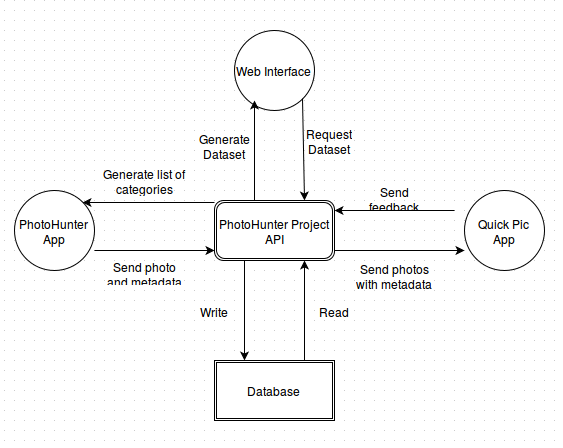
\includegraphics[width=\textwidth,height=\textheight,keepaspectratio]{ss_flowchart}
\end{frame}

\subsection{Researchers Interface}

\begin{frame}{Researchers Interface}
  \centering
  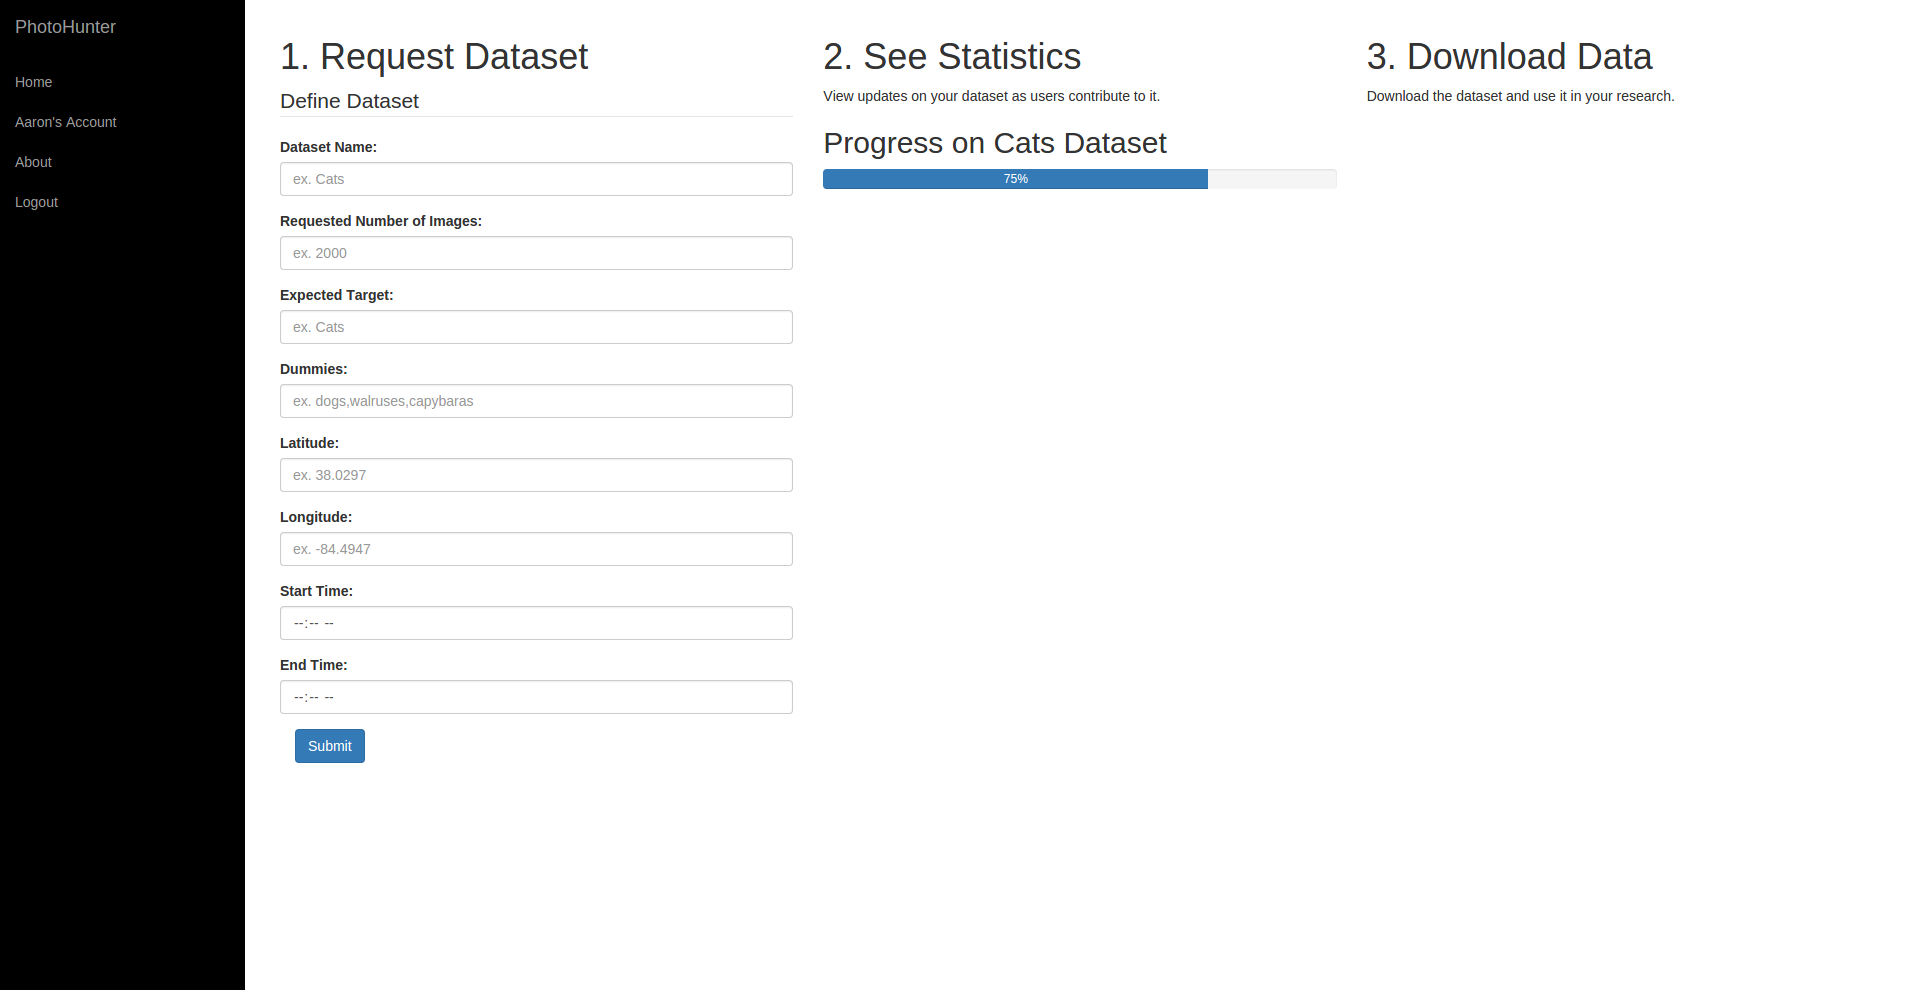
\includegraphics[width=\textwidth,height=\textheight,keepaspectratio]{researchers}
\end{frame}

\subsection{PhotoHunter}

\begin{frame}{PhotoHunter}
  \begin{columns}[c]
    \begin{column}{0.5\columnwidth}
      \centering
      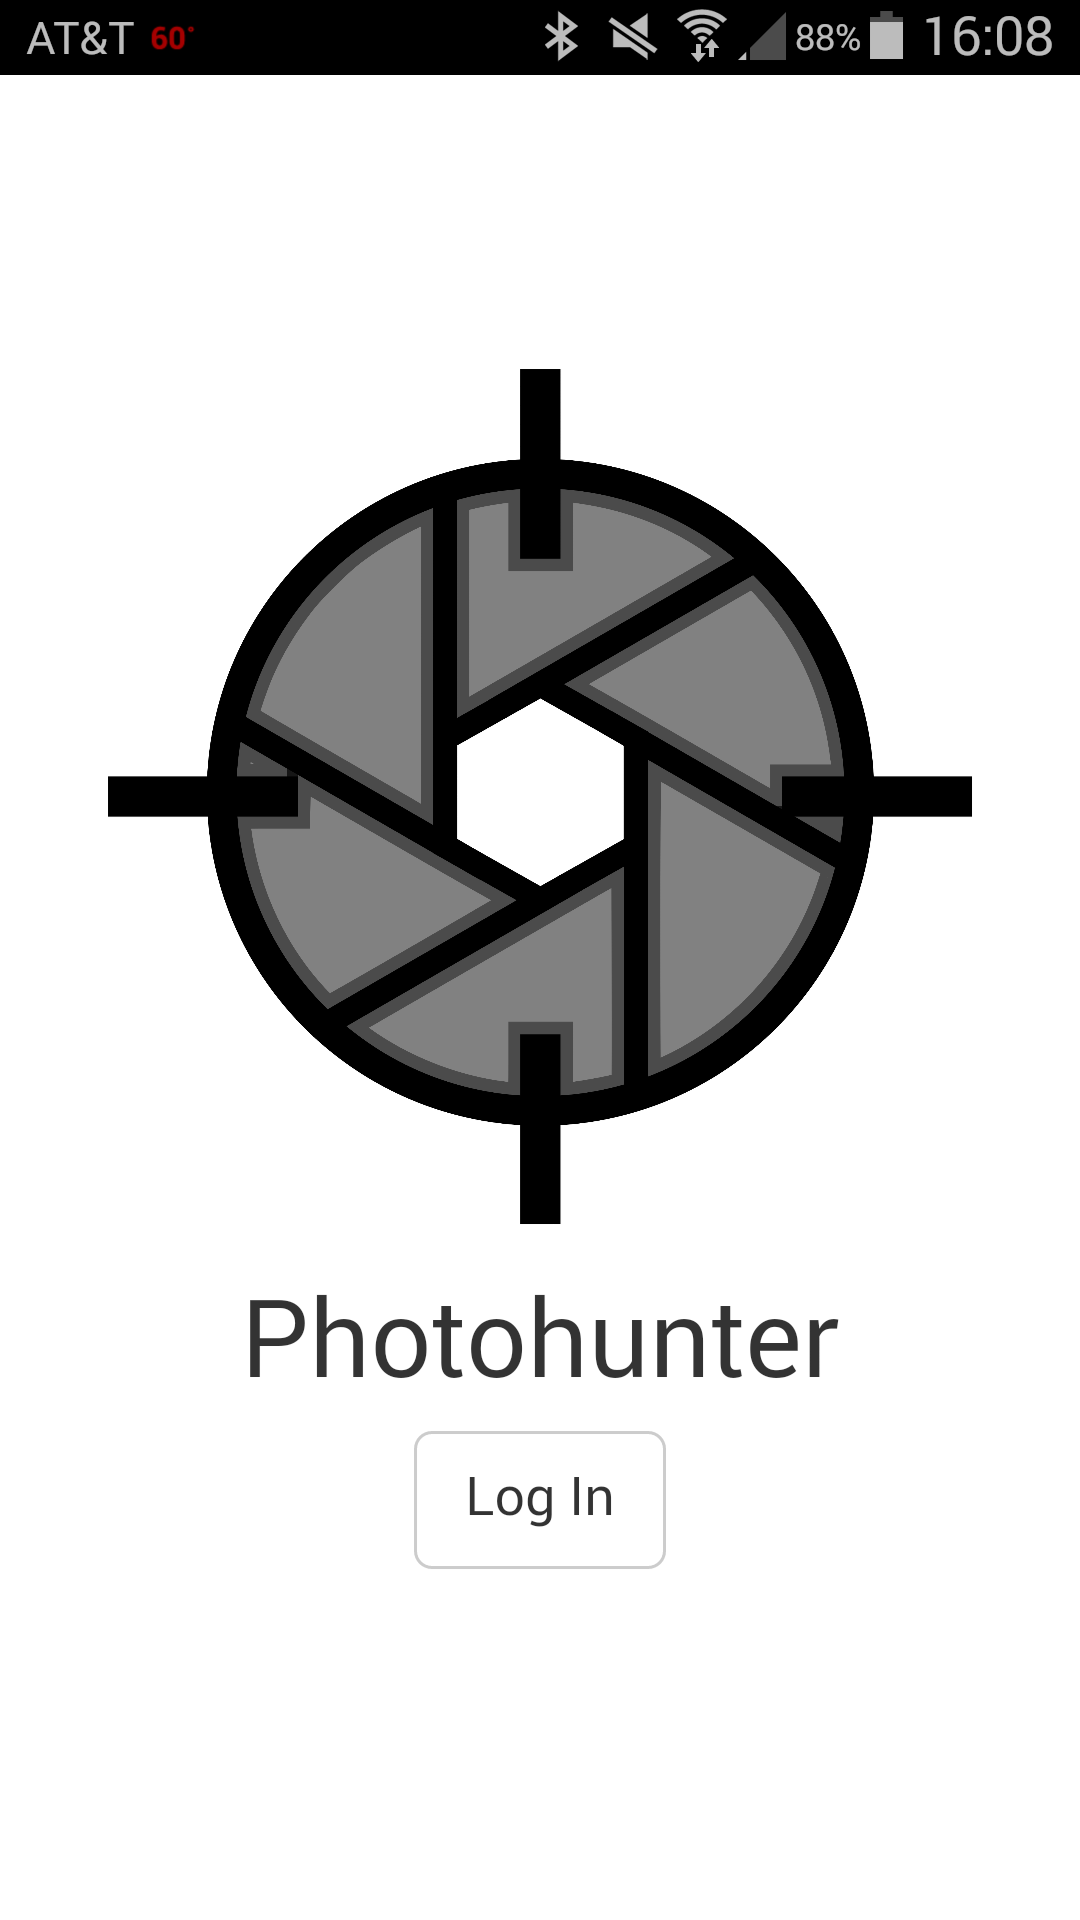
\includegraphics[width=\textwidth,height=\textheight,keepaspectratio]{photohunter/login}
    \end{column}
    \begin{column}{0.5\columnwidth}
      \centering
      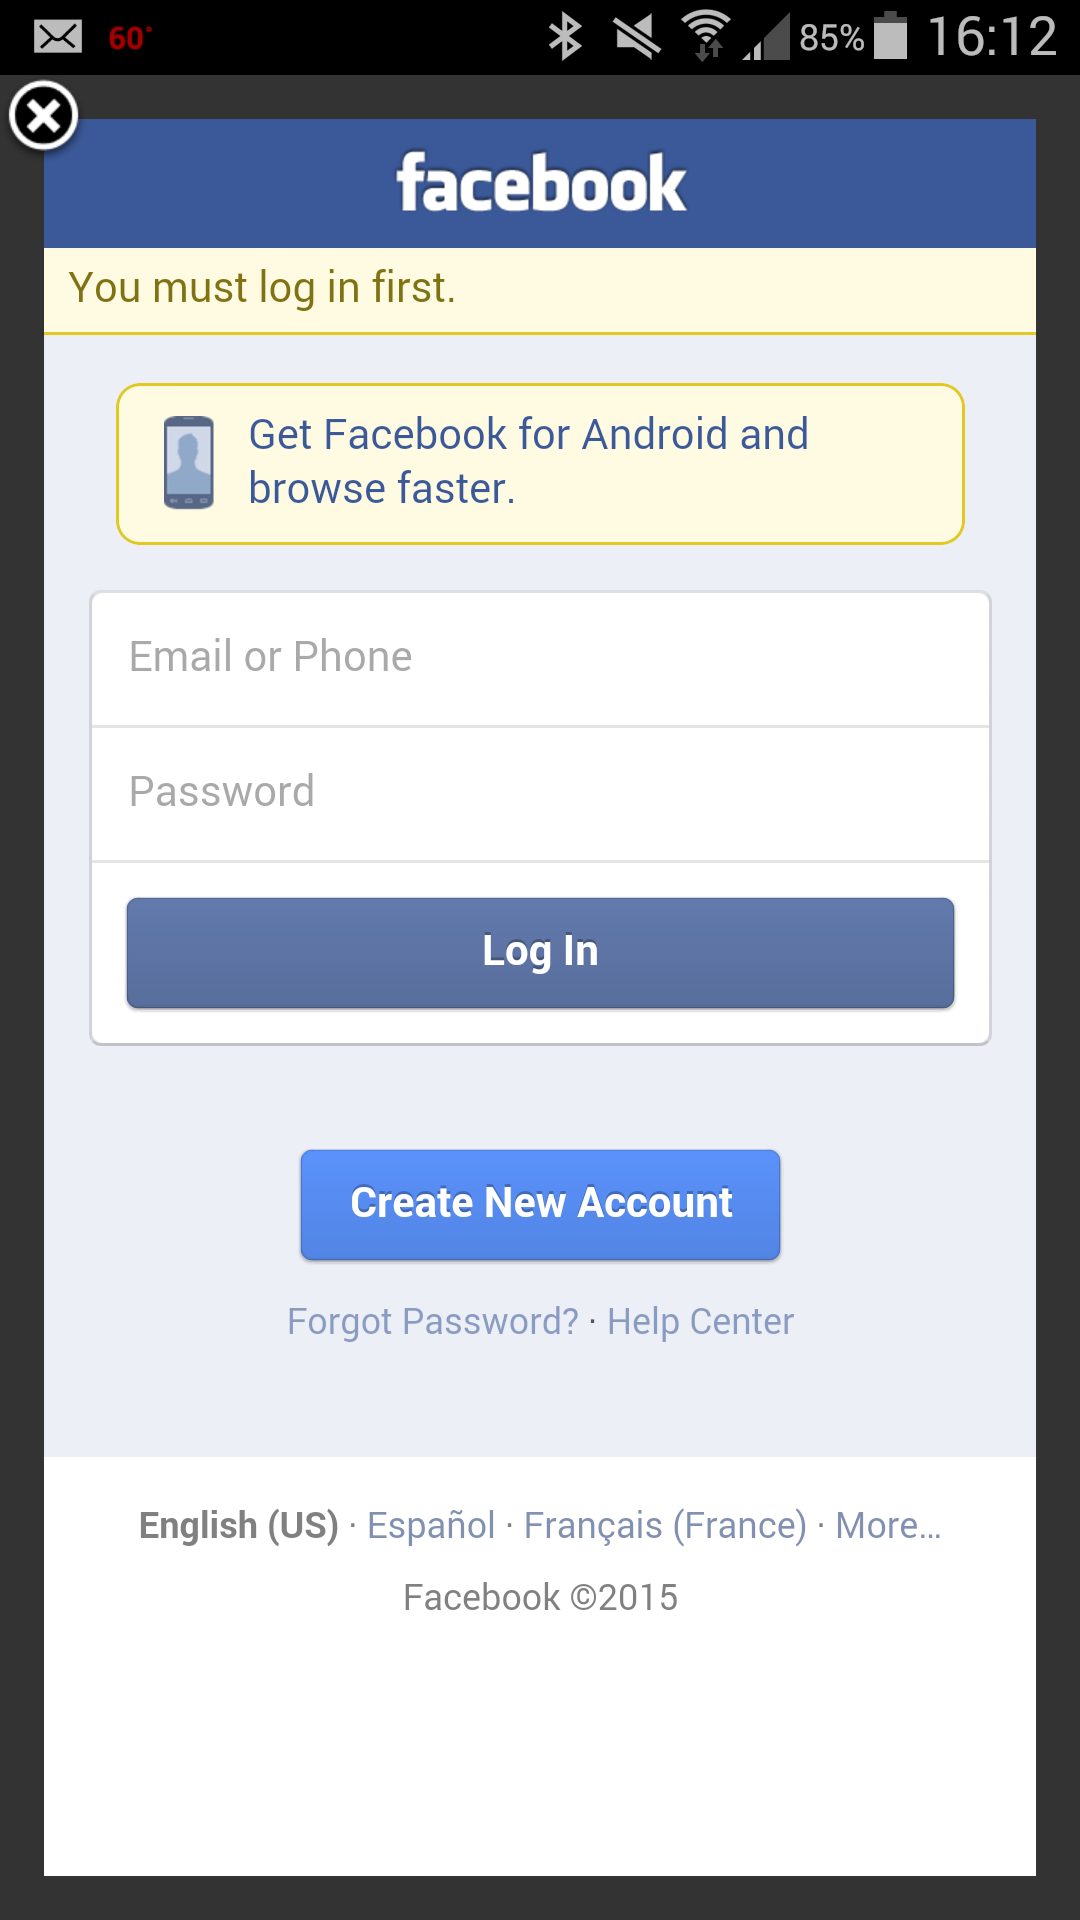
\includegraphics[width=\textwidth,height=\textheight,keepaspectratio]{photohunter/fb}
    \end{column}
  \end{columns}
\end{frame}

\begin{frame}{PhotoHunter}
  \begin{columns}[c]
    \begin{column}{0.3\columnwidth}
      \centering
      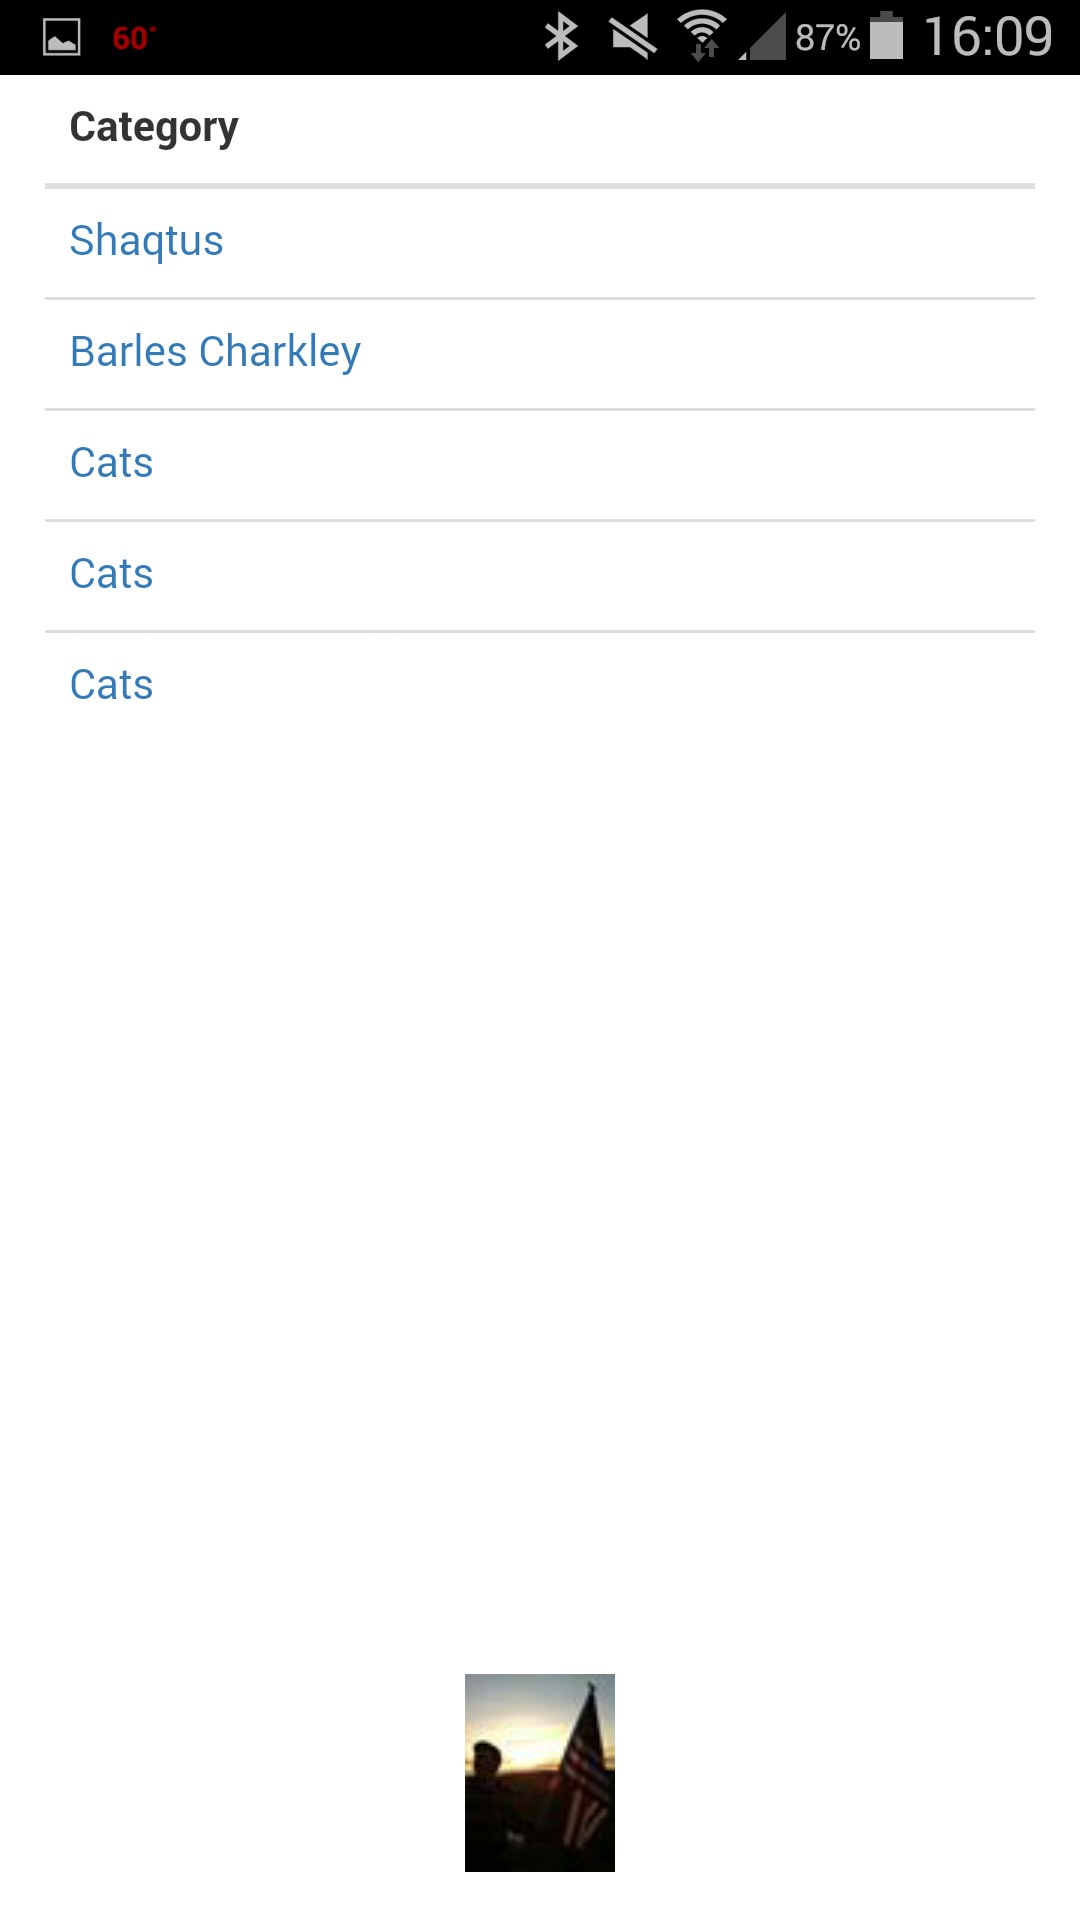
\includegraphics[width=\textwidth,height=\textheight,keepaspectratio]{photohunter/list}
    \end{column}
    \begin{column}{0.3\columnwidth}
      \centering
      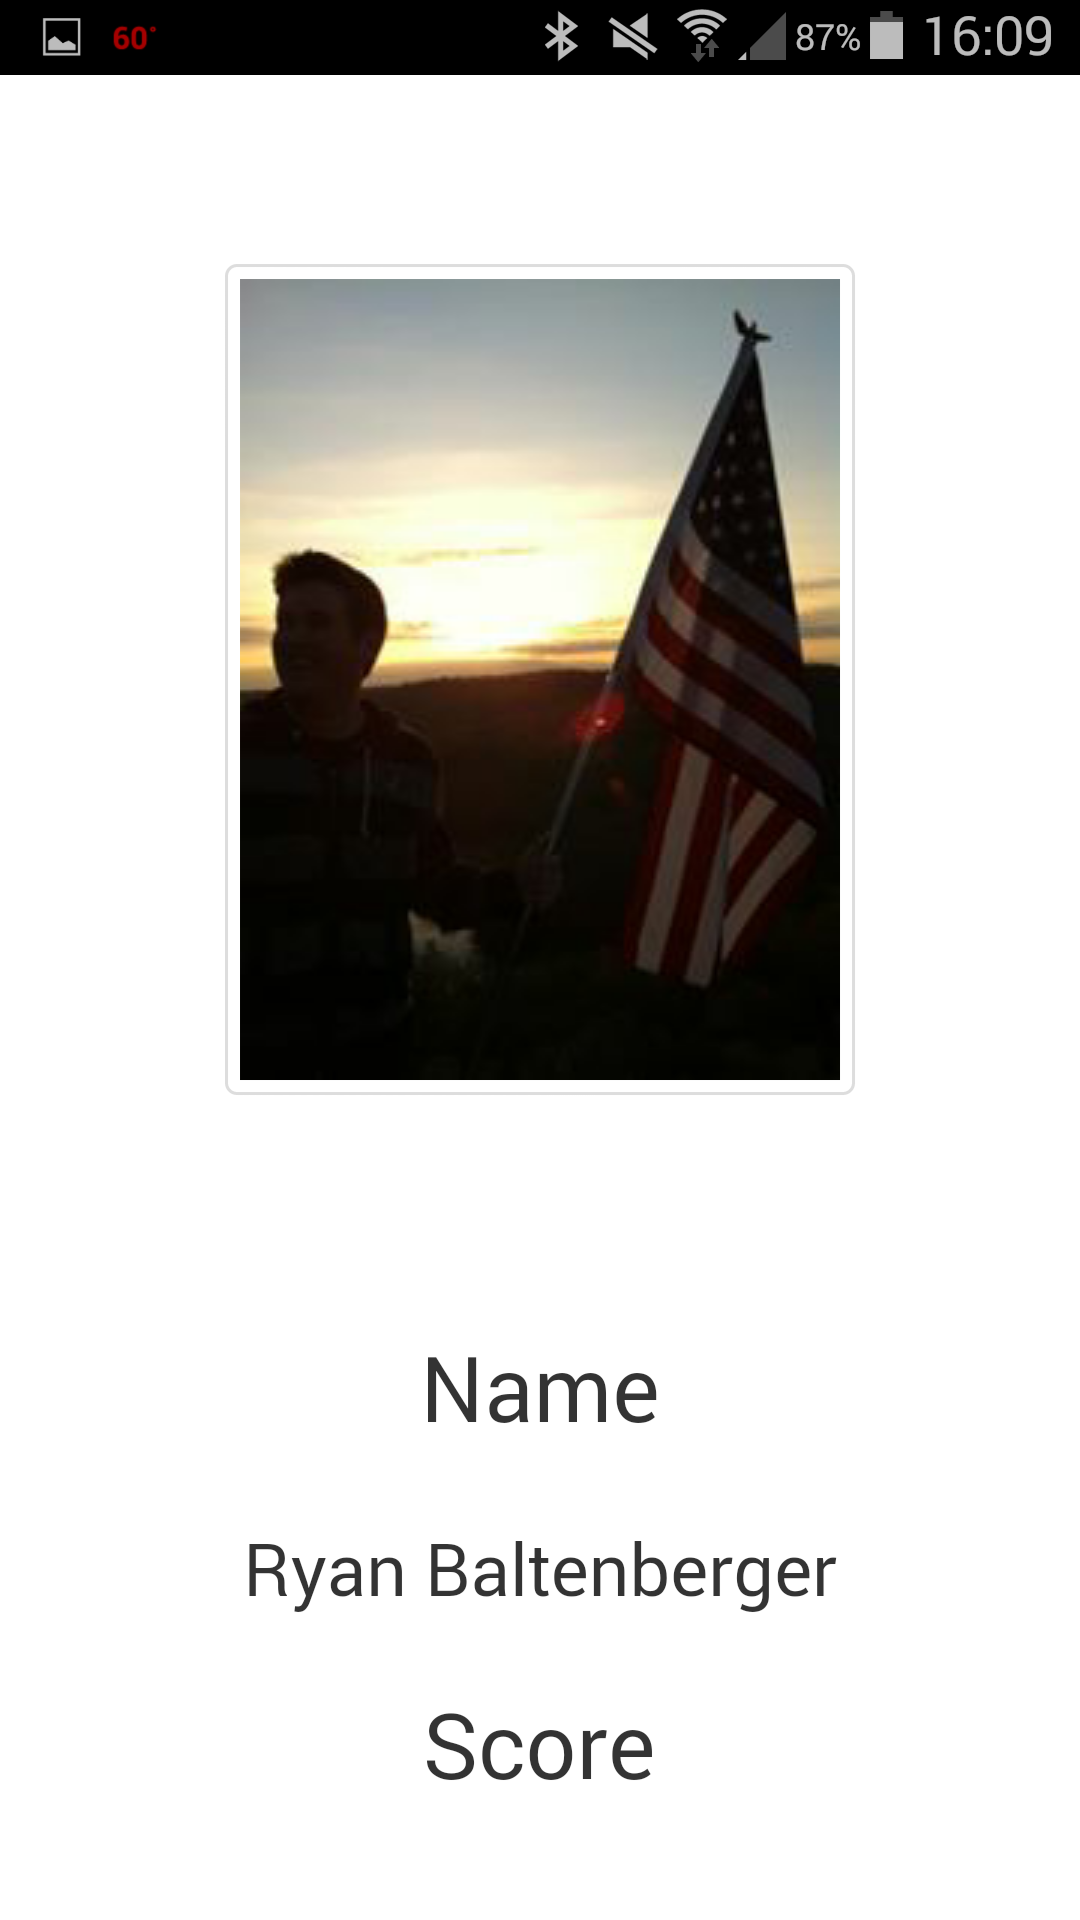
\includegraphics[width=\textwidth,height=\textheight,keepaspectratio]{photohunter/user}
    \end{column}
    \begin{column}{0.3\columnwidth}
      \centering
      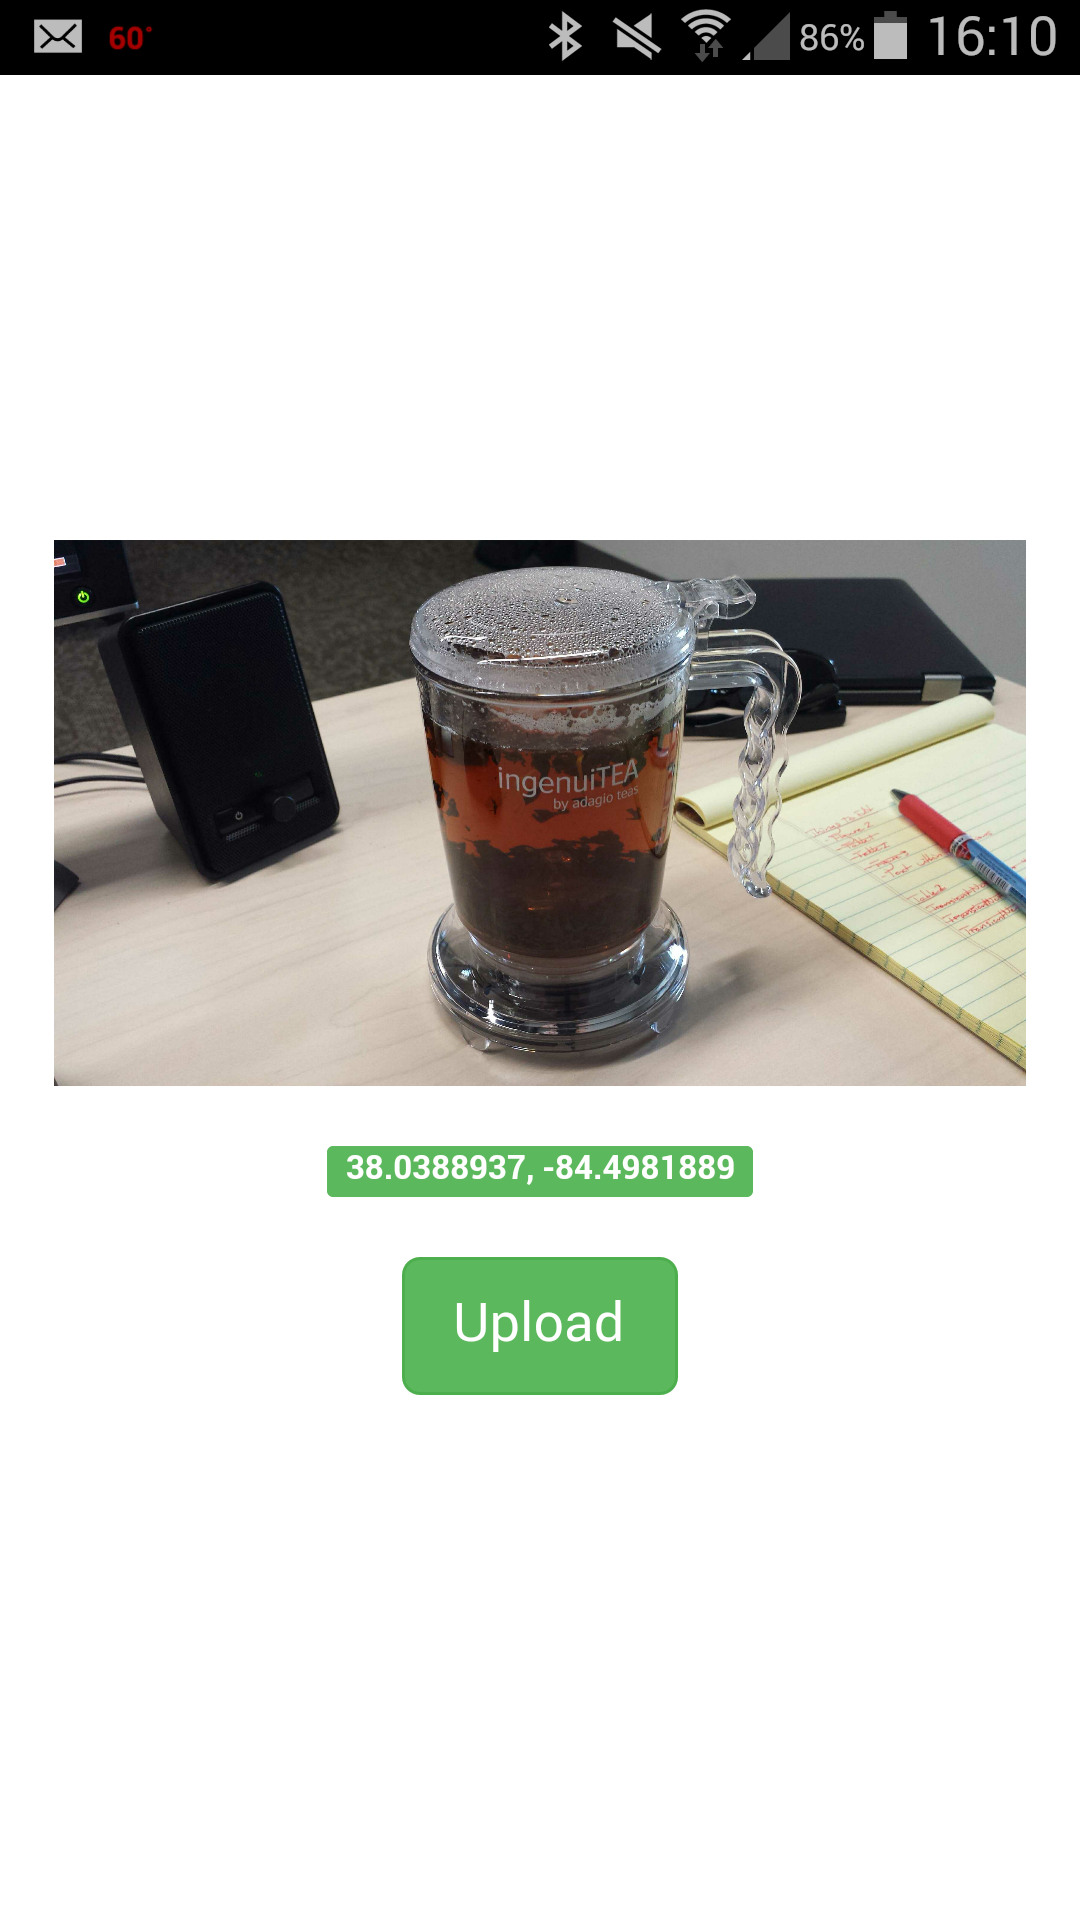
\includegraphics[width=\textwidth,height=\textheight,keepaspectratio]{photohunter/submit}
    \end{column}
  \end{columns}
\end{frame}

\subsection{QuickPic}

\begin{frame}{QuickPic}
  \begin{columns}[c]
    \begin{column}{0.3\columnwidth}
      \centering
      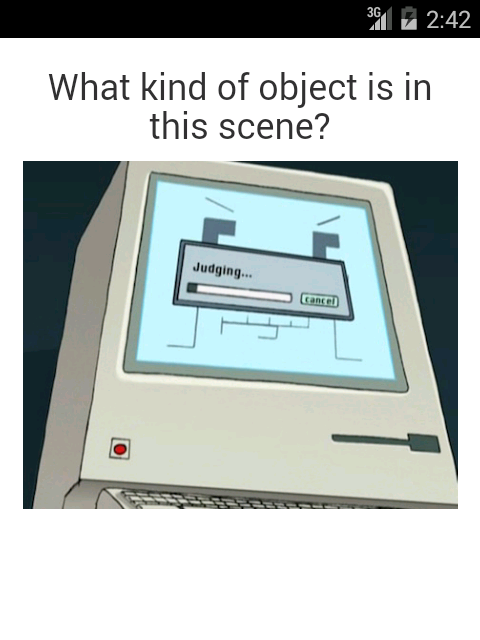
\includegraphics[width=\textwidth,height=\textheight,keepaspectratio]{ss_quickpic_image}
    \end{column}
    \begin{column}{0.3\columnwidth}
      \centering
      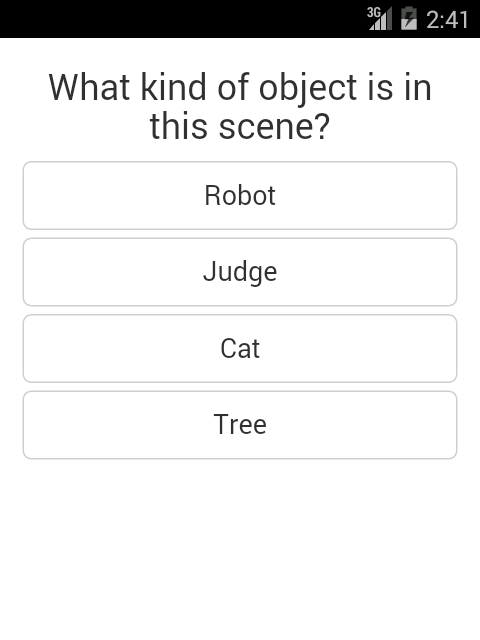
\includegraphics[width=\textwidth,height=\textheight,keepaspectratio]{ss_quickpic_options}
    \end{column}
    \begin{column}{0.3\columnwidth}
      \centering
      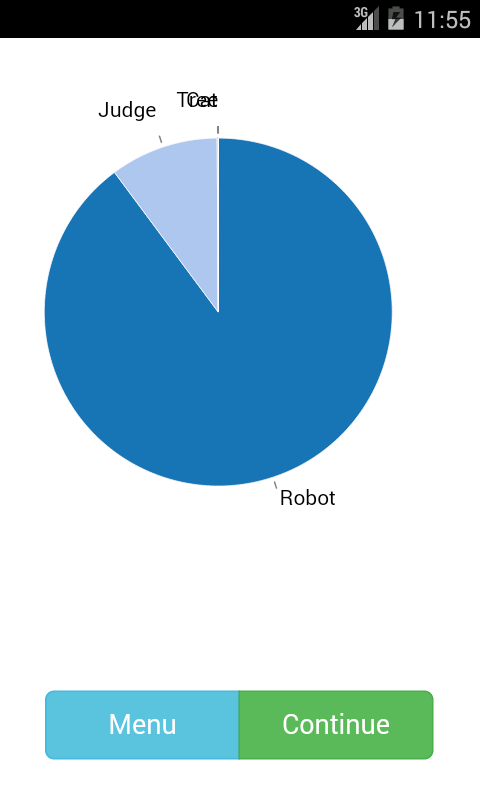
\includegraphics[width=\textwidth,height=\textheight,keepaspectratio]{ss_quickpic_stats}
    \end{column}
  \end{columns}
\end{frame}

\subsection{Backend}

\begin{frame}{ER Diagram}
  \centering
  \includegraphics[width=\textwidth,height=\textheight,keepaspectratio]{er}
\end{frame}

% Discuss problems, and your solutions
% Discuss lessons learned while doing the project
\section{Lessons Learned}

\begin{frame}{Lessons Learned}
	\begin{itemize}

		\item Learning Cordova and app development without previous experience

    \item Developing web application with Go and PostgreSQL/PostGIS with limited experience

		\item Integrating with the Facebook API

		\item Piecing together bits of documentation from multiple projects

	\end{itemize}
\end{frame}

% Discuss your initial assumptions about the project compared to what you know now
% Does the project match what the customer initially wanted, how did it evolve
\section{Assumptions and Evolution}

\begin{frame}{Assumptions and Evolution}
	\begin{itemize}

		\item Initial concept included only one app (PhotoHunter)

		\item QuickPic came from need to verify image categories (but was going to
					be a part of the PhotoHunter app at first)

		\item API came from need to interface with both apps and the web backend

	\end{itemize}
\end{frame}

% Changes requested by the customer, or changes to specifications due to implementation
\section{Changes}

\begin{frame}{Changes}
	\begin{itemize}

		\item Leaderboards and testing/deploying on multiple platforms were moved to
					be stretch goals if time permitted

		\item Cordova was chosen to make deploying to multiple platforms later on
					easier

		\item Interfacing with PostgreSQL and Go created unexpected issues with the database

    \item The researcher interface and API were merged into one package

	\end{itemize}
\end{frame}

% Discuss future enhancements, usage
\section{The Future!}

\begin{frame}{The Future!}
	\begin{itemize}

		\item Leaderboard Integration

		\item Deploy to other platforms

		\item Security checks on apps and web interface

		\item Market the apps and get users to use them/test them

		\item Make apps more "game-y"

	\end{itemize}
\end{frame}

\frame{\centering Thanks!}

\end{document}
